\section{Durchführung}
\label{sec:Durchführung}

In der ersten Messreihe wird für Rohre drei verschiedener Durchmesser die
Frequenzverschiebung $\Delta \nu$ für drei verschiedene Dopplerwinkel
bei sechs verschiedenen Strömungsgeschwindigkeiten mit einer 2\,Mhz-Sonde gemessen.

Dafür wird ein Dopplerprisma mit Dopplerwinkeln von 15°, 30° und 60° verwendet,
um die Winkel konstant zu halten. Ein Dopplerprisma ist in Abbildung \ref{fig:dopplerprisma}
dargestellt.
\begin{figure}
  \centering
  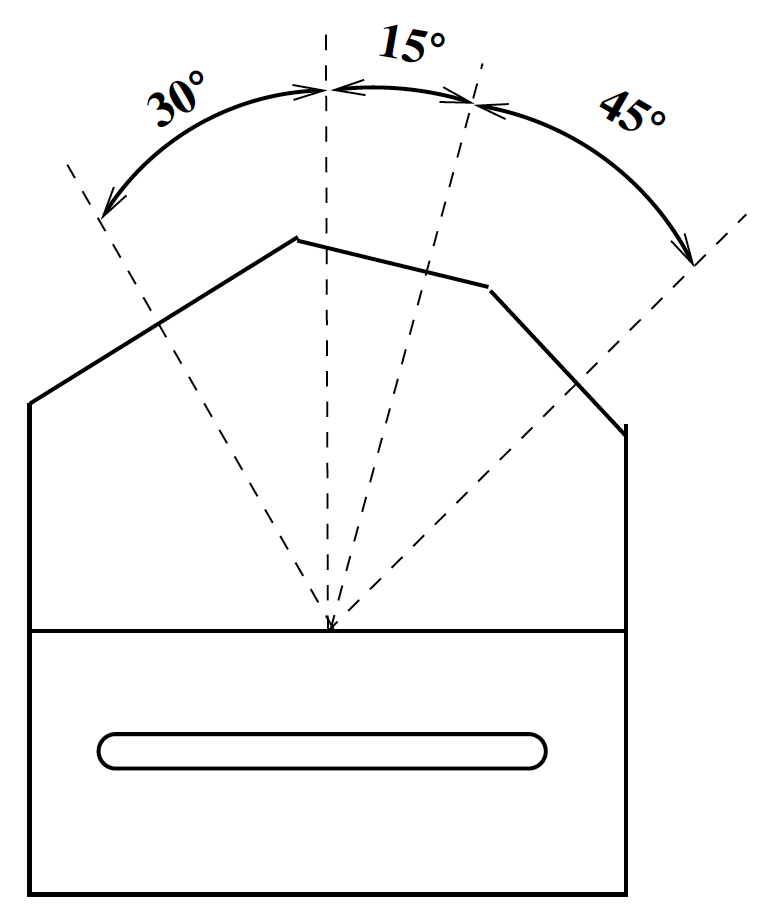
\includegraphics[width=5cm]{data/dopplerprisma.png}
  \caption{Skizze eines Dopplerprismas\,\cite{Versuchsanleitung}.}
  \label{fig:dopplerprisma}
\end{figure}
Die Ultraschall-Sonde ist an einen Computer angeschlossen und die Daten werden
von einem Programm verarbeitet.

Die rohrspezifischen Dopplerprismen werden zunächst mit Koppelgel an das jeweilige
Rohr gekoppelt. Außerdem wird Koppelgel auf die Ultraschallsonde aufgetragen.
An einer Pumpe kann die Strömungsgeschwindigkeit eingestellt werden. Nun wird
die Frequenzverschiebung für ein
Rohr mit einem Innendurchmesser von 16\,mm, ein Rohr mit einem Innendurchmesser von
10\,mm und ein Rohr mit einem Innendurchmesser von 7\,mm gemessen. Da die gemessenen
Frequenzverschiebungen nicht diskret sind, wird aus dem Programm der Mittelwert
für diese abgelesen und notiert. Bei der Messung ist stets darauf zu achten, die
Größen, die gerade gemessen werden auch in das Programm einzutragen, damit dieses
die Werte korrekt verarbeiten kann.

In einer weiteren Messreihe wird daraufhin das Strömungsprofil des eines Rohres mit
einem Innendurchmesser von 10\,mm für zwei verschiedene Strömungsgeschwindigkeiten
gemessen. Dafür wird an einem Messgerät für die Sonde die Tiefe, in der gemessen wird
eingestellt und aus dem Programm der Mittelwert und die Standardabweichung abgelesen.
